\subsection{Horse Owner}

\subsubsection{Login}

\textbf{Role:} Spectator

\begin{itemize}
    \item \textbf{Function trigger:} The spectator enters account credentials to log in.

    \item \textbf{Function description:}
    \begin{itemize}
        \item \textbf{Purpose:}
        \begin{enumerate}
            \item Verify the spectator's identity.
            \item Grant access to spectator functionalities.
        \end{enumerate}

        \item \textbf{Data processing:}
        \begin{enumerate}
            \item The spectator enters username and password.
            \item The system validates credentials.
            \item The system identifies the SPECTATOR role.
            \item The system creates a login session.
        \end{enumerate}
    \end{itemize}
\end{itemize}

\textbf{Screen layout:}

\begin{figure}[H]
    \centering
    
\includegraphics[width=0.7\textwidth]{figures/web_application/spectator/login.png}
    \caption{Spectator Login}
\end{figure}

\subsubsection{Prediction Management}

\textbf{Role:} Spectator

\begin{itemize}
    \item \textbf{Function trigger:} The spectator navigates to the "Du doan Tran dua" (Predict Race) menu.

    \item \textbf{Function description:}
    \begin{itemize}
        \item \textbf{Purpose:}
        \begin{enumerate}
            \item Allow the spectator to submit a new race ranking prediction to earn reward points.
            \item Allow the spectator to view, edit, or delete their existing prediction history.
        \end{enumerate}

        \item \textbf{Data processing:}
        \begin{enumerate}
            \item \textbf{For creating a new prediction:}
            \begin{itemize}
                \item The spectator selects a race, selects a horse, and chooses the predicted finishing rank from the dropdown menus.
                \item The spectator clicks the "Gui du doan" button.
                \item The system validates the prediction data and saves it to the database.
            \end{itemize}
            \item \textbf{For managing prediction history:}
            \begin{itemize}
                \item The system retrieves and displays the spectator's accumulated reward points and prediction history list (including Race, Horse, Predicted Rank, Result, and Actions).
                \item If the race status is pending ("Cho ket qua"), the system allows the spectator to click "Sua" (Edit) or "Xoa" (Delete) to update their prediction.
                \item If the race has ended, the actions are disabled ("Da khoa"), and the system updates the prediction status ("DUNG" / "SAI") along with the spectator's total reward points.
            \end{itemize}
        \end{enumerate}
    \end{itemize}
\end{itemize}

\textbf{Screen layout:}

\begin{figure}[H]
    \centering
    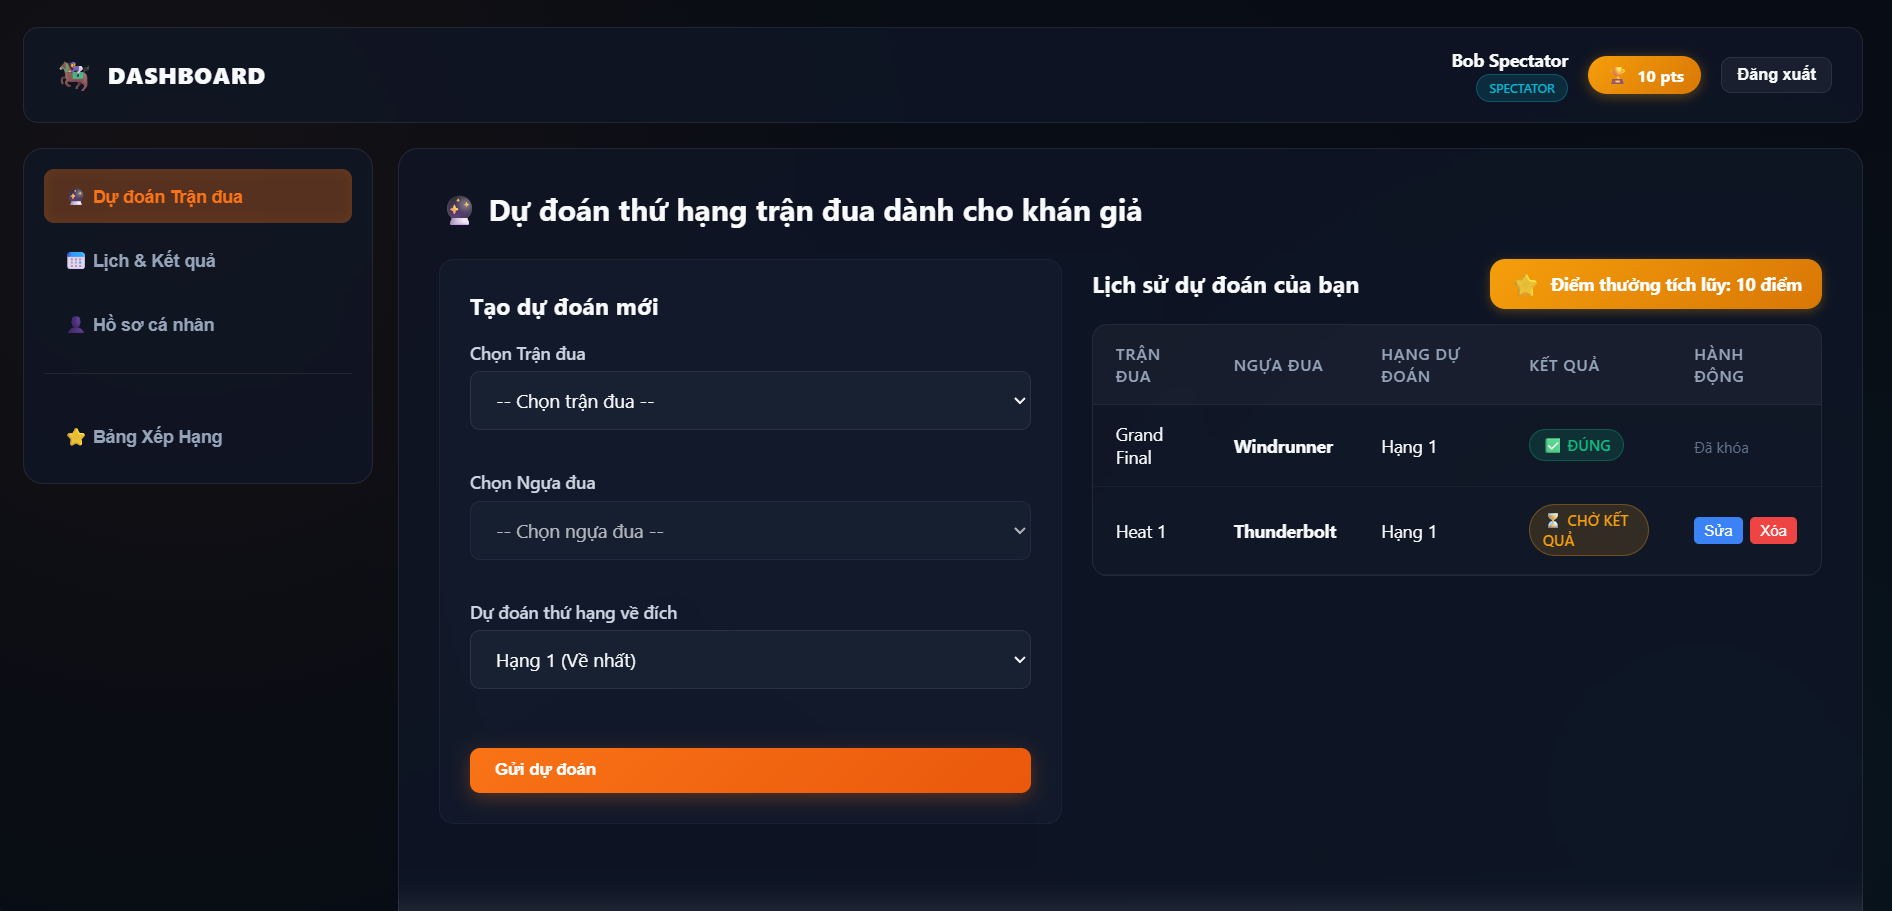
\includegraphics[width=0.7\textwidth]{figures/web_application/spectator/prediction.png}
    \caption{Spectator Prediction}
\end{figure}

\subsubsection{View Schedule and Results}

\textbf{Role:} Spectator

\begin{itemize}
    \item \textbf{Function trigger:} The spectator navigates to the "Lich \& Ket qua" (Schedule \& Results) menu.

    \item \textbf{Function description:}
    \begin{itemize}
        \item \textbf{Purpose:}
        \begin{enumerate}
            \item Allow the spectator to view the list of upcoming race schedules.
            \item Allow the spectator to view the detailed results and rankings of completed races.
        \end{enumerate}

        \item \textbf{Data processing:}
        \begin{enumerate}
            \item \textbf{For upcoming race schedules ("Lich thi dau sap dien ra"):}
            \begin{itemize}
                \item The system retrieves and displays scheduled races with status "SCHEDULED".
                \item Information includes: Race name (e.g., Heat 1), referee name, date, time, distance, track condition, and the list of participating horses ("Danh sach tham gia") with their respective jockeys.
            \end{itemize}
            \item \textbf{For completed race results ("Ket qua cac tran da ket thuc"):}
            \begin{itemize}
                \item The system retrieves and displays finished races with status "HOAN THANH".
                \item For each completed race (e.g., Grand Final), the spectator can expand to view the detailed ranking table including: Rank ("Hang"), Horse ("Ngua dua"), Jockey, Score ("Diem"), and Notes ("Ghi chu").
            \end{itemize}
        \end{enumerate}
    \end{itemize}
\end{itemize}

\textbf{Screen layout:}

\begin{figure}[H]
    \centering
    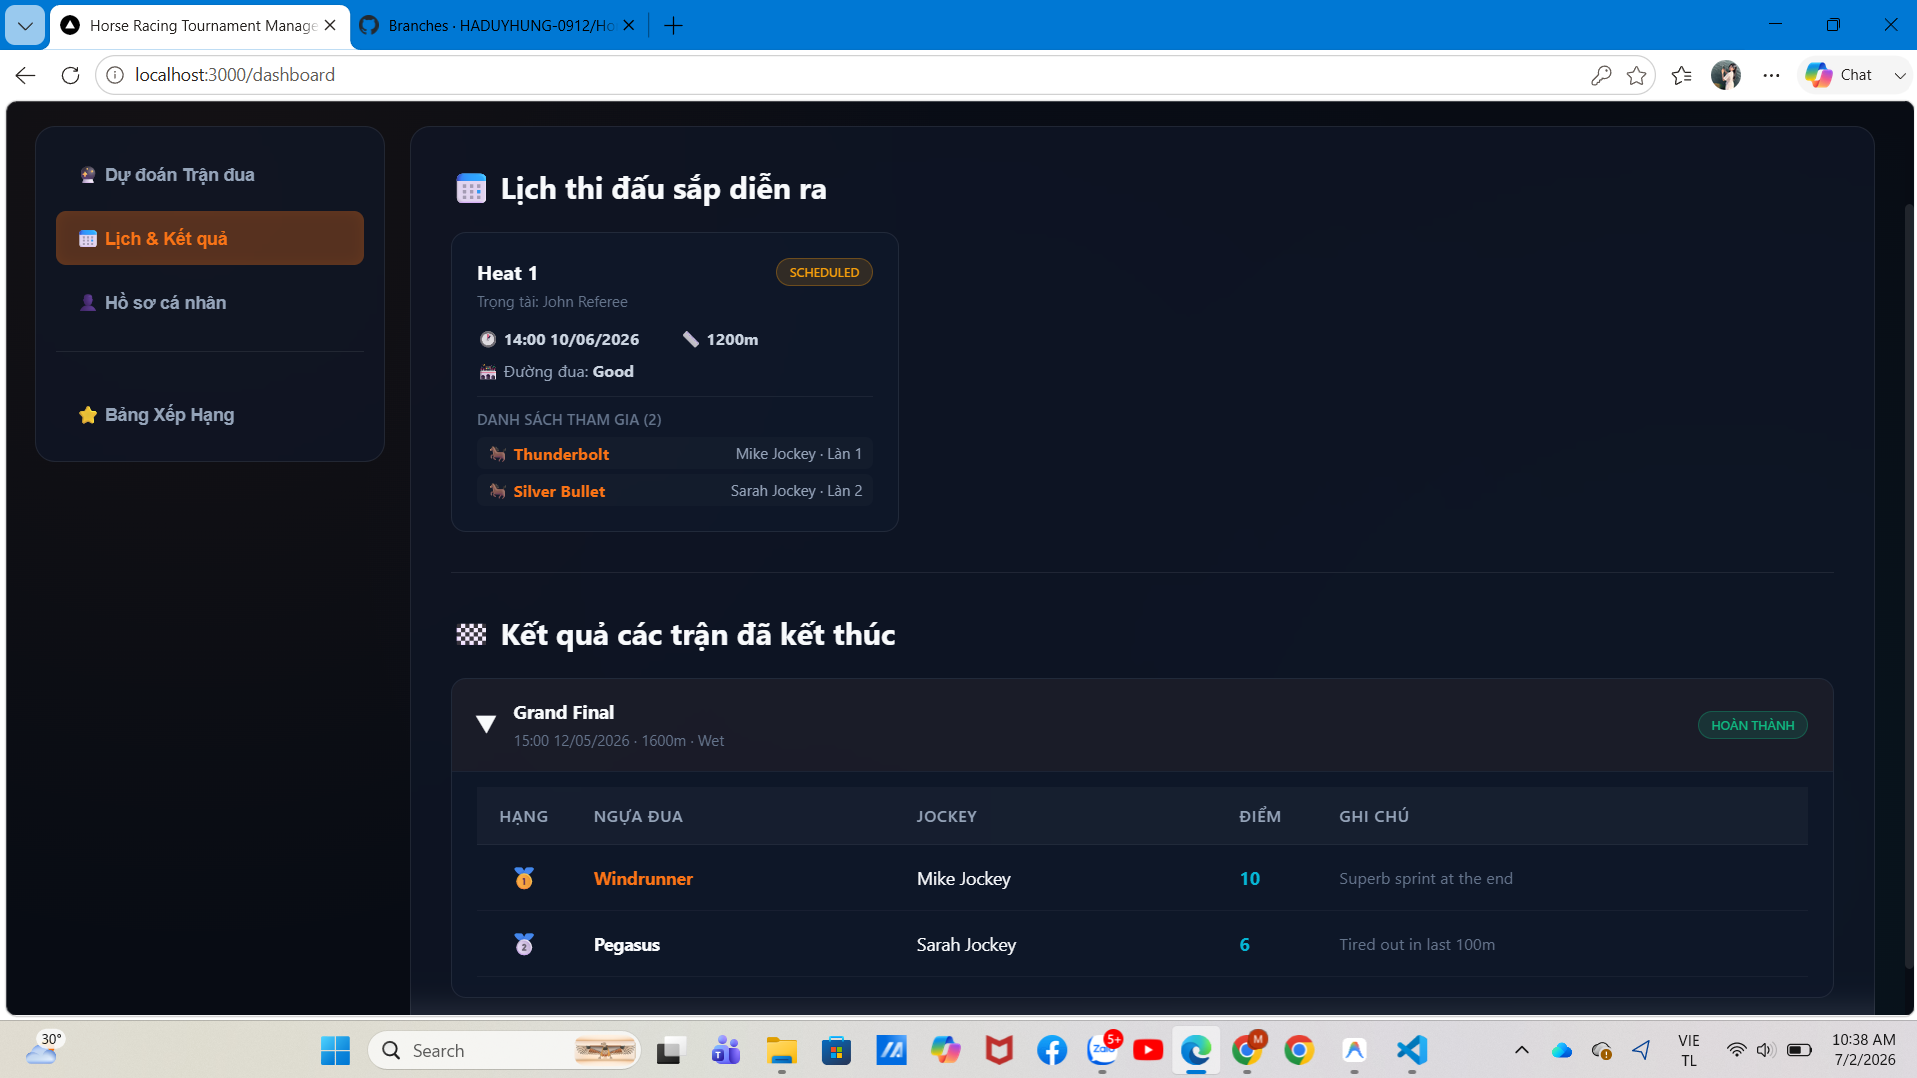
\includegraphics[width=0.7\textwidth]{figures/web_application/spectator/schedule_and_results.png}
    \caption{View Schedule and Results}
\end{figure}

\subsubsection{Personal Profile}

\textbf{Role:} Spectator

\begin{itemize}
    \item \textbf{Function trigger:} The spectator navigates to the "Ho so ca nhan" (Personal Profile) menu.

    \item \textbf{Function description:}
    \begin{itemize}
        \item \textbf{Purpose:}
        \begin{enumerate}
            \item Allow the spectator to view and update their personal profile information.
            \item Display the spectator's prediction statistics, performance overview, and recent prediction history.
        \end{enumerate}

        \item \textbf{Data processing:}
        \begin{enumerate}
            \item \textbf{For updating profile information:}
            \begin{itemize}
                \item The spectator can view and edit the following fields: Full Name ("Ho va Ten"), Email, Phone Number ("So dien thoai"), Avatar URL ("URL Anh dai dien"), Favorite Horse Breed ("Giong ngua yeu thich"), and Favorite Jockey ("Nai ngua yeu thich").
                \item The spectator clicks the "Cap nhat thong tin" button.
                \item The system validates the entered data and updates the profile details in the database.
            \end{itemize}
            \item \textbf{For viewing statistics and history:}
            \begin{itemize}
                \item The system retrieves and displays statistical insights ("Thong ke \& Thanh tich") including: Current Rank ("Thu hang hien tai"), Total Predictions ("Tong so tran du doan"), Accuracy Rate ("Ty le chinh xac"), and Reward Points ("Diem thuong").
                \item The system retrieves and lists the recent prediction history ("Lich su du doan gan day") with columns: Race Name ("Ten tran dua"), Selected Horse ("Ngua da chon"), Time ("Thoi gian"), Status ("Trang thai"), and Reward Points ("Diem thuong").
            \end{itemize}
        \end{enumerate}
    \end{itemize}
\end{itemize}

\textbf{Screen layout:}

\begin{figure}[H]
    \centering
    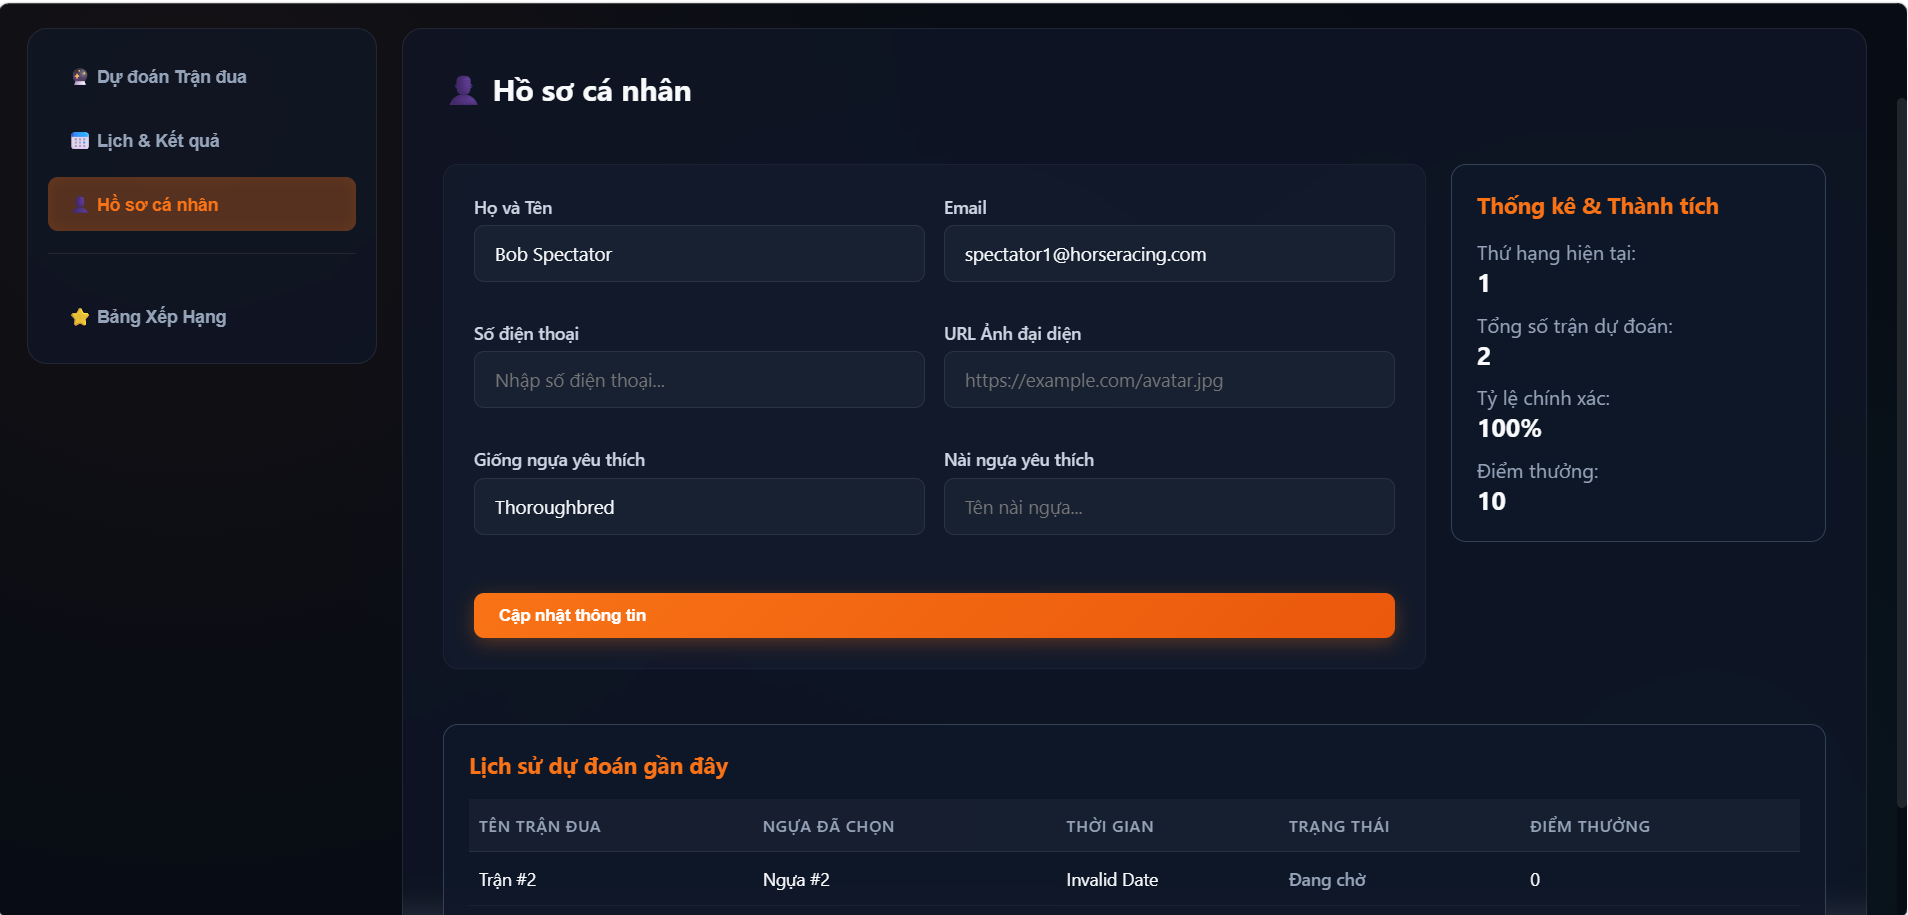
\includegraphics[width=0.7\textwidth]{figures/web_application/spectator/personal_profile.png}
    \caption{View Personal Profile}
\end{figure}

\subsubsection{Leaderboard}

\textbf{Role:} Spectator

\begin{itemize}
    \item \textbf{Function trigger:} The spectator navigates to the "Bang Xep Hang" (Leaderboard) menu.

    \item \textbf{Function description:}
    \begin{itemize}
        \item \textbf{Purpose:}
        \begin{enumerate}
            \item Allow the spectator to view the official competition rankings of horses and jockeys, filtered by tournament.
            \item Allow the spectator to view the top 10 spectators with the highest prediction accuracy scores.
        \end{enumerate}

        \item \textbf{Data processing:}
        \begin{enumerate}
            \item \textbf{For Horse \& Jockey Leaderboard ("Ngua \& Jockey" tab):}
            \begin{itemize}
                \item The spectator can filter rankings by tournament ("Loc theo giai dau") including options: All ("Tat ca"), Summer Championship 2026, or Spring Derby 2026.
                \item The system retrieves and displays the Horse Ranking table ("Xep hang Ngua dua") including columns: Rank ("Hang"), Horse Name ("Ten ngua"), and Accumulated Points ("Diem tich luy").
                \item The system retrieves and displays the Jockey Ranking table ("Xep hang Jockey") including columns: Rank ("Hang"), Jockey Name ("Ten jockey"), and Accumulated Points ("Diem tich luy").
            \end{itemize}
            \item \textbf{For Top Spectators Leaderboard ("Khan gia xuat sac" tab):}
            \begin{itemize}
                \item The system retrieves and displays the top 10 spectators with the highest prediction scores ("Top 10 Khan gia co diem du doan cao nhat").
                \item The leaderboard table includes columns: Rank ("Hang"), Spectator Name ("Khan gia"), Favorite Horse Breed ("Giong ngua yeu thich"), and Accumulated Points ("Diem tich luy").
            \end{itemize}
        \end{enumerate}
    \end{itemize}
\end{itemize}

\textbf{Screen layout:}

\begin{figure}[H]
    \centering
    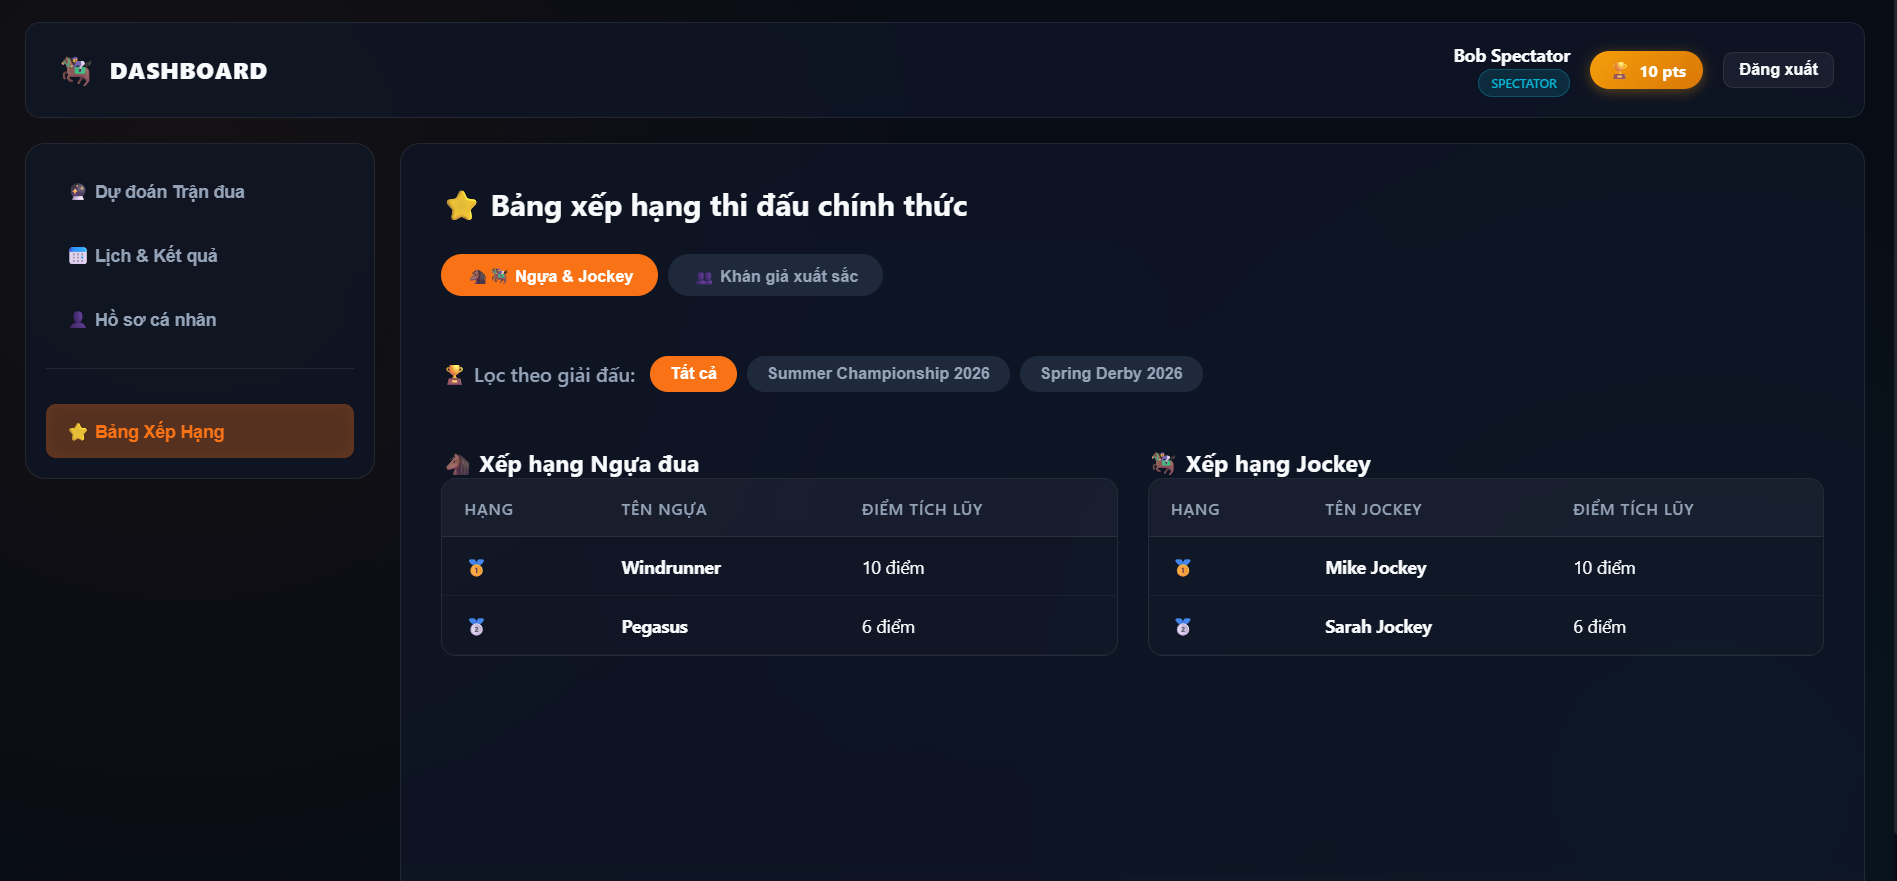
\includegraphics[width=0.7\textwidth]{figures/web_application/spectator/horse_and_jockey_leaderboard.png}
    \caption{Official Competition Leaderboard for Horses and Jockeys}
\end{figure}

\textbf{Screen layout:}

\begin{figure}[H]
    \centering
    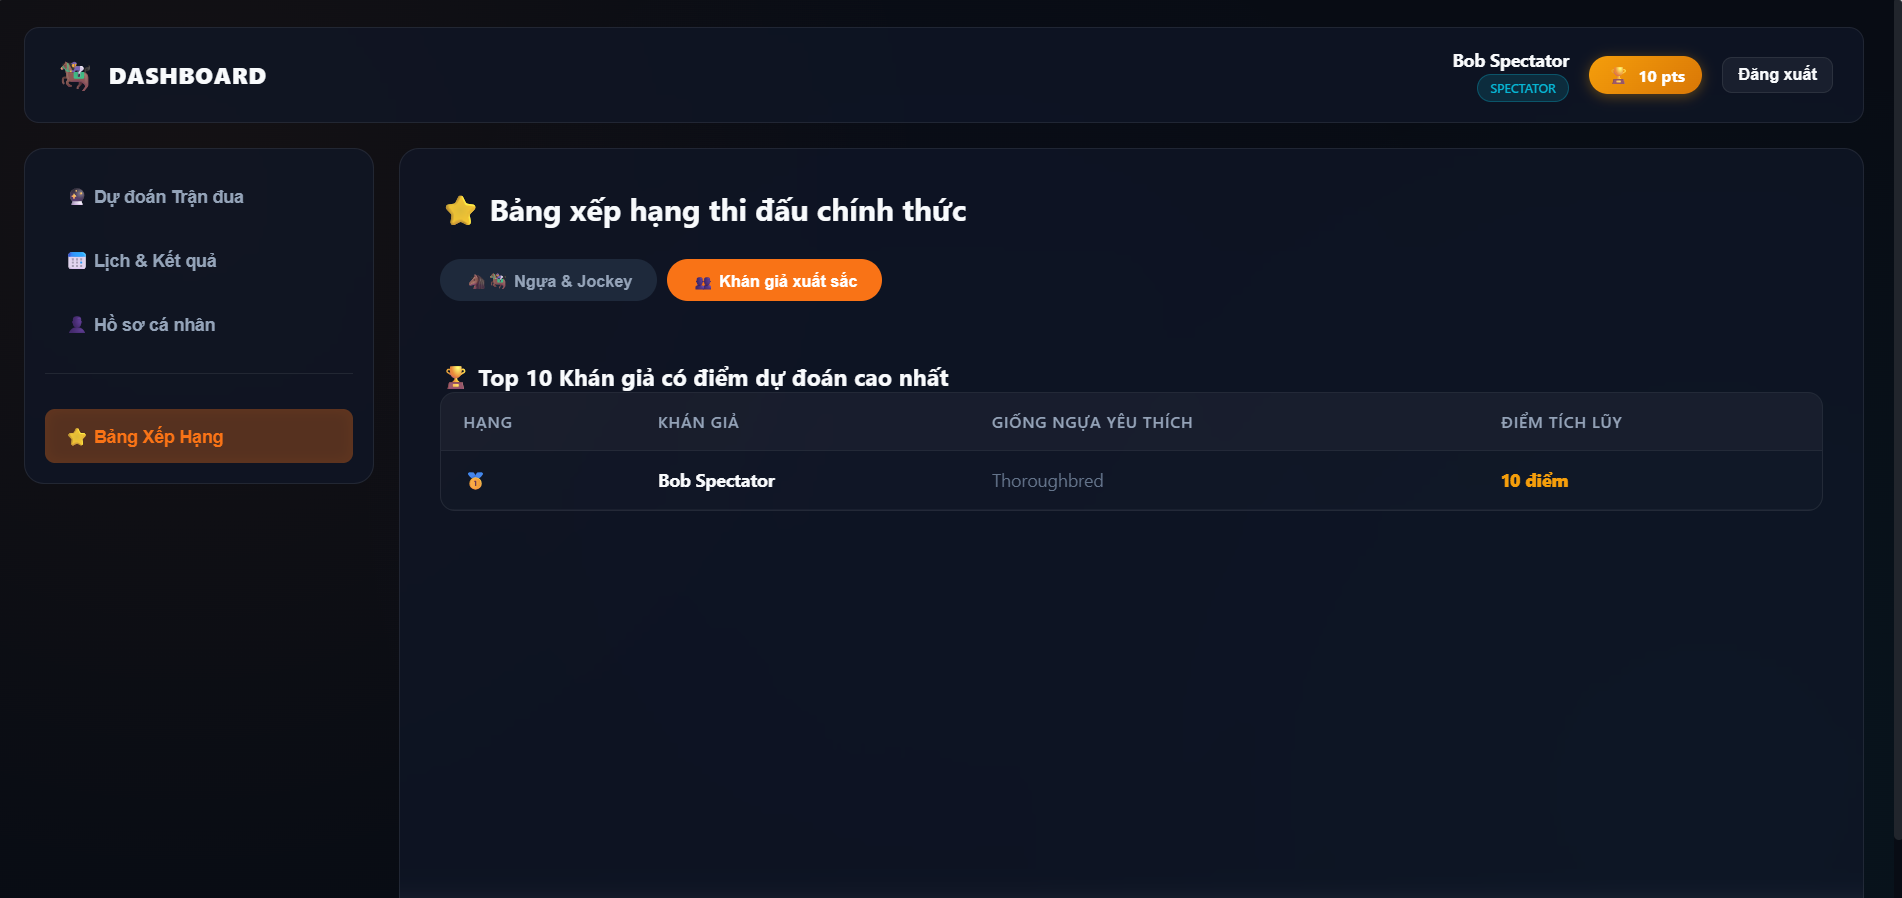
\includegraphics[width=0.7\textwidth]{figures/web_application/spectator/spectators_leaderboard.png}
    \caption{View Top 10 Spectators Prediction Leaderboard}
\end{figure}
